%pa_nonlinearities
%\documentclass[11pt,twoside,a4paper,notitlepage]{scrartcl} 
\documentclass[11pt,oneside,a4paper]{scrartcl} 
%==============================================
% Version 0.0 DD-MMM_YYYY JM
%==============================================

% PACKAGES

\usepackage{color}
\usepackage{amsmath}
\usepackage{amsfonts}
\usepackage{amssymb}
\usepackage{marvosym}
\usepackage{eufrak}
\usepackage{steinmetz}
\usepackage{color}
\usepackage{listings}
\usepackage{subfigure}
\usepackage{url}
\usepackage[utf8x]{inputenc}

\RequirePackage{palatino}\fontfamily{ppl}

\definecolor{mygreen}{RGB}{50, 140, 140}

\usepackage[colorlinks=true,linkcolor=mygreen]{hyperref}		% must be the last package

% LEVEL OF HEADERS

\setcounter{secnumdepth}{2}
\setcounter{tocdepth}{2}


%\evensidemargin=-0.3cm
%\oddsidemargin=1.5cm
\textheight=23.0cm

\usepackage{pdfsync}


% JM standard macros
%===================
%
% Equation, figures, and tables
%
\newcommand{\EQ}[1]{\begin{equation}\label{Eq:#1}}
\newcommand{\EE}{\end{equation}}
\newcommand{\Equation}[1]{Equation~(\ref{Eq:#1})}
\newcommand{\Eq}[1]{Eq.~(\ref{Eq:#1})}
\newcommand{\EqRef}[1]{(\ref{Eq:#1})}
\newcommand{\Figure}[1]{Figure~\ref{Fig:#1}}
\newcommand{\Fig}[1]{Fig.~\ref{Fig:#1}}
\newcommand{\Table}[1]{Table~\ref{Tab:#1}}
\newcommand{\Page}[1]{p.~\pageref{#1}}
%
% Protected from hyphenation:
%
\newcommand{\EISCAT}{\mbox{EISCAT}}
%
% Units
%
\newcommand{\Hz}{\ensuremath{\mathrm{Hz}}}
\newcommand{\degr}{\ensuremath{^\circ}}
\newcommand{\mpersec}{\ensuremath{\rm{m\,s^{-1}}}}
\newcommand{\kmpersec}{\ensuremath{\rm{km\,s^{-1}}}}
\newcommand{\mperss}{\ensuremath{\rm{m\,s^{-2}}}}
\newcommand{\ms}{\ensuremath{\mathrm{ms}}}
\newcommand{\cm}{\ensuremath{\mathrm{cm}}}
\newcommand{\us}{\ensuremath{\rm{\mu s}}}
%
% Math
%
\newcommand{\ip}[2]{\ensuremath{\langle{#1},{#2}\rangle}}
\newcommand{\norm}[1]{\ensuremath{\|#1\|}}
\newcommand{\est}[1]{\ensuremath{\widehat{#1}}}
\newcommand{\abs}[1]{\ensuremath{|#1|}}
\newcommand{\Abs}[1]{\ensuremath{\left|#1\right|}}
\newcommand{\cc}[1]{\ensuremath{{#1}^*}}
%\newcommand{\cc}[1]{\ensuremath{\overline{#1}}}
\newcommand{\ave}[1]{\ensuremath{\overline{#1}}}
\newcommand{\real}{\ensuremath{\rm{Re}}}
\newcommand{ \diric } {\ensuremath { \mathrm {diric} }} 
\newcommand{ \Expe } {\ensuremath { { {\rm E} } }} 
\newcommand{ \Exp }[1] {\ensuremath {\mathrm e ^ {#1}}} 
\newcommand { \sinc } {\ensuremath { \mathrm {sinc} }} 
\newcommand{\vc}[1]{\ensuremath{\mathbf{#1}}}
\newcommand{\uv}[1]{\ensuremath{\mathbf{\hat {#1}}}}
%
% MF
%
\newcommand{\SNR}{{\rm{SNR}}}
\newcommand{\prog}[1]{\textsc{#1}}
\newcommand{\Tc}{\ensuremath{T_\mathrm{c}}}
\newcommand { \SNRN } {\ensuremath { \mathrm { SNR_N } }}
\newcommand { \ENR } {\ensuremath { \mathrm { ENR } }}
\newcommand { \vRR } {\ensuremath { v_\mathrm{RR}  }}
\newcommand { \vD } {\ensuremath { v_\mathrm{D}  }}
\newcommand { \Tsys } {\ensuremath { T_\mathrm{sys} }}
\newcommand { \MF } {\ensuremath { \mathrm { MF } }} 
\newcommand { \AF } {\ensuremath { \mathrm { AF } }} 
\newcommand { \FMF } {\ensuremath { \mathrm {FMF} }} 
\newcommand { \FAF } {\ensuremath { \mathrm { FAF } }} 

\newcommand { \Dp } {\ensuremath { D_\mathrm { p } }} 
\newcommand { \Trep } {\ensuremath { T_\mathrm {rep} }} 
\newcommand { \Ratio } {\ensuremath { \mathrm {Ratio} }} 
%
% Misc
%
\newcommand{\BULLETS}{\begin{itemize}}
\newcommand{\ENDBULLETS}{\end{itemize}}
\newcommand{\ENUMERATE}{\begin{enumerate}}
\newcommand{\ENDENUMERATE}{\end{enumerate}}
\newcommand { \FRepI } {\cite{Markkanen2002}} 
\newcommand{\RCS}{\ensuremath{\mathrm{RCS}}}
\newcommand{\deff}{\ensuremath{d_\mathrm{eff}}}
\newcommand { \fRF } {\ensuremath {f_{\mathrm {RF}}}} 
\newcommand { \GE } {\ensuremath {G_{\mathrm {E}}}} 
\newcommand { \gE } {\ensuremath {\mathcal{D}_{\mathrm {E}}}} 
\newcommand { \Gref } {\ensuremath {G_{\mathrm {ref}}}} 
\newcommand{\Four}[1]{\ensuremath{\tilde {#1}}}
\newcommand { \D } {\ensuremath {\mathcal{D}}} 

\newcommand { \mr }[1] {\ensuremath {\mathrm{#1}}} 

%
% Coloured text
%
\newcommand{\BL}[1]{\color{blue}#1 \color{black}}
\newcommand{\RED}[1]{\color{red}#1 \color{black}}

% end JM standard macros


\newif\ifpdf
\ifx\pdfoutput\undefined
\pdffalse
\else
\pdfoutput=1
\pdftrue
\fi

\ifpdf
\usepackage[pdftex]{graphicx}
\else
\usepackage{graphicx}
\fi

% =============================================================================
% The following GOOD advice is from the page
% http://mintaka.sdsu.edu/GF/bibliog/latex/floats.html 
% by Andrew T. Young.
% =============================================================================
% Alter some LaTeX defaults for better treatment of figures:
    % See p.105 of "TeX Unbound" for suggested values.
    % See pp. 199-200 of Lamport's "LaTeX" book for details.
    %   General parameters, for ALL pages:
    \renewcommand{\topfraction}{0.9}	% max fraction of floats at top
    \renewcommand{\bottomfraction}{0.8}	% max fraction of floats at bottom
    %   Parameters for TEXT pages (not float pages):
    \setcounter{topnumber}{2}
    \setcounter{bottomnumber}{2}
    \setcounter{totalnumber}{4}     % 2 may work better
    \setcounter{dbltopnumber}{2}    % for 2-column pages
    \renewcommand{\dbltopfraction}{0.9}	% fit big float above 2-col. text
    \renewcommand{\textfraction}{0.07}	% allow minimal text w. figs
    %   Parameters for FLOAT pages (not text pages):
    \renewcommand{\floatpagefraction}{0.7}	% require fuller float pages
	% N.B.: floatpagefraction MUST be less than topfraction !!
    \renewcommand{\dblfloatpagefraction}{0.7}	% require fuller float pages

	% remember to use [htp] or [htpb] for placement
% =============================================================================



%--------------------------------------------------------------
% Title page components
%--------------------------------------------------------------

\title{
\vspace{4cm}\BL{
PfP Array
}\\
\vspace{0.2cm}
\Large
}

\author{
J Markkanen\\
}

%\date{DD-MONTH-YYYY}
\date{\today}



%##############################################################################
\begin{document}
%##############################################################################

\ifpdf
\DeclareGraphicsExtensions{.pdf, .jpg,.png}
\else
\DeclareGraphicsExtensions{.eps, .jpg}
\fi

\section*{Power amplifier nonlinearities}

\subsubsection*{Polynomial model}
%%
One way to model the non-linear amplifier behaviour is to write the output $y(t)$ corresponding to an input signal $x(t)$ as an $n$-degree polynomial such as
\EQ{10}
	y = \mathcal{P}[x] = a_1 x + a_2 x^2 + a_3 x^3 + a_4 x^4 + a_5 x^5 \,,
\EE
with constant, real-valued coefficients $a_n$. 

For high power PA driven near saturation, even the 5-degree polynomial model \Eq{10} can be quite poor and more complicated expressions are needed for realistic simulation. These involve adding higher degree terms, say up to degree 7, and, crucially, adding what are called ``memory terms''. The memory terms take into account that the output $y(t)$ does not depend just on the input at a single instant of time $t$, but, filter like, on the preceding times $t-\delta t$ also. The resulting expression for $y(t)$ is a Volterra series. 

We will inspect consequences of the polynomial model when the signal $x(t)$ consists of one or two sinusoidal signals. Typical calculations in standard sources like the two book of Cripps\footnote{
Steve C. Cripps, RF Power Amplifiers for Wireless Communications, Second Edition, Artech House, 2006, and Steve C. Cripps, Advanced Techniques in RF Power Amplifier Design, Artech House, 2002. 
},
involve tiresome real-valued trigonometric algebra. Here, we will work with complex exponentials $A\Exp{ j\omega t}$ instead. This leads to simpler calculations, and, more importantly, gives results immediately in a form that is directly related to signal spectra as could be inspected with a spectrum analyser.

\subsubsection*{Single-tone test signal}
%%
The simplest input test signal to show effects of PA nonlinearities is a single sinusoid,
\begin{eqnarray}
	x_1(t) &=& 2b_0 \cos( \omega_1 t + \phi) \label{Eq:A10} \\
			&=& b \Exp{j\omega_1 t} + \cc b \Exp{-j\omega_1 t} \label{Eq:A15}
\end{eqnarray}
where $b = b_0\Exp{j\phi}$. Its spectrum is shown in top panel of \Fig{pa_1tone}. By (discrete) spectrum, we mean the sequence $\left(Y(n\omega_1)\right)$ of the complex coefficients in the normal Fourier series representation of the periodic function, e.g.
\EQ{A18}
	y(t) = \sum_{n = -\infty}^\infty Y(n\omega_1) \Exp{j n \omega_1 t} \,.
\EE
 
We will use a the fifth degree polynomial model \Eq{10} for the PA output. All the individual terms $a_n x^n(t)$ of the polynomial are also periodic functions, with the same period $P = 2\pi/\omega_1$ as $x_1(t)$,  so have a Fourier series representation. The spectra of the five terms $a_n x^n$ are shown schematically in Panels~(b)--(f) of \Fig{pa_1tone}; the spectrum of the complete model of \Eq{10} is the sum of these.  

For \Fig{pa_1tone}, we calculated the spectra of the terms $a_n x^n$ by applying the binomial formula
\[
	(A+B)^n = \sum_{k=0}^n \binom{n}{k} A^{n-k}B^k 
\]
to \Eq{A15},
\EQ{A22}
	x_1^n
	=
	\left(b \Exp{j \omega_1 t} + \cc b \Exp{-j\omega_1 t}\right)^n
	= 
	\sum_{k=0}^n \binom{n}{k} b^{n-k}({\cc b})^k \Exp{j (n - 2k)\omega_1 t} \,.
\EE
The binomial coefficients are most conveniently picked from the Pascal Triangle, Table~\ref{pascal_triangle}. 
\begin{table}[t]
\caption{Pascal Triangle up to degree five.}
\begin{center}
\footnotesize
\begin{tabular}{rccccccccccc}\hline\\
$n=0$:&    &    &    &    &    &  1\\\noalign{\smallskip\smallskip}
$n=1$:&    &    &    &    &  1 &    &  1\\\noalign{\smallskip\smallskip}
$n=2$:&    &    &    &  1 &    &  2 &    &  1\\\noalign{\smallskip\smallskip}
$n=3$:&    &    &  1 &    &  3 &    &  3 &    &  1\\\noalign{\smallskip\smallskip}
$n=4$:&    &  1 &    &  4 &    &  6 &    &  4 &    &  1\\\noalign{\smallskip\smallskip}
$n=5$:&  1 &    &  5 &    & 10 &    & 10 &    &  5 &    &  1\\
\end{tabular}
\normalsize
\end{center}
\label{pascal_triangle}
\end{table}
%
For example, the third degree term $a_3x_1^3$ can now immediately written down with help of \Eq{A22} in a standard Fourier-series form
\begin{eqnarray}
	a_3x_1^3(t) &=&	a_3b^3 \cdot \Exp{j3\omega_1 t}
					+ 3a_3 {\Abs b}^2 {b} \cdot \Exp{j\omega_1 t}
					+ 3a_3 {\Abs b}^2 {\cc b} \cdot \Exp{-j\omega_1 t}
					+ a_3b^3\cdot \Exp{-j3\omega_1 t} 
					\label{Eq:A20}
\end{eqnarray}
from which its spectrum as shown in Panel~(d) of \Fig{pa_1tone} can be readily read off. 

With $a_n$ real-valued, the spectra in \Fig{pa_1tone} have hermitian symmetry and so we have not bothered to explicitly write down the amplitudes of the negative frequency spectral components in Panels~(d)--(f). 

But we have allowed the Fourier-amplitudes ($b$ and $\cc b)$ of the input signal to be complex-valued, to account for an initial non-zero phase of $x_1(t)$. This is because we want to see \footnote{ 
We want to see this explicitly, because Cripps, and others, set the initial phase of $x_1(t)$ to zero without any justification. Admittedly, justification is simple, but I still worth mentioning. For a single-tone input signal $x_1$, an initial phase is equivalent to a shift of time origin. In our PA model, the same shift then pertains the output signal $y(t)$ also. From the theory of Fourier series, the spectral magnitude squared is the mean power at that frequency---mean calculated over the period of the periodic signal---and such a quantity obviously cannot depend on the time origin. An other justification is that from the theory of Fourier series we know that a time shift causes only a phase factor in spectral domain, and thus cannot affect the magnitude (of the total) output signal spectrum.}
%
explicitly how it comes about in the math that the spectral power distribution $\Abs{Y(n\omega)}^2$ of the total signal does not depend on the initial phase of the input signal, even though the complex-valued $Y(m\omega)$ get complex-valued contribution from many $a_k x^k$ terms. 

Panel~(b) of \Fig{pa_1tone} shows the ideal, desired output $y(t) = a_1 x(t)$ of the PA. The ideal output is identical in form to the input and differs from the input only by the voltage gain factor $a_1$. Also, the output depends linearly on the input in the ideal case. The non-linear effects are illustrate in subsequent panels which show the spectral power spreading to unwanted frequencies, increasing the output bandwidth. With the single-tone input signal, the unwanted frequencies are integer multiples $n\omega_1$ of the input frequency $\omega_1$, and are called harmonics of the fundamental frequency $\omega_1$. 

\Figure{pa_1tone} suggests, and \Eq{A22} proves, that in the polynomial model, an even-degree term $a_n x_1^n$ produces spectral components at all even-order harmonic frequencies from $0$ to $\pm n\omega_1$. Similarly, an odd-$n$ term $a_n x_1^n$ produce spectral components at all odd harmonic frequencies from $-n\omega_1$ to 
$+n\omega_1$. 

Of particular concern in typical PA application are the odd-degree non-linear terms which pile unwanted spectral power, with non-linear dependence on input signal amplitude $b$, directly on top of the fundamental spectral component at $\omega_1$.

From \Eq{A22}, we get an explicit formula for the total output spectral component at the fundamental frequency in $N$'th degree model, for the single-tone input signal. In the binomial expansion, only odd-degree terms $n = 2m+1$ contribute at $1\omega_1$. Of these, the actually contributing term has $k$ such that $(2m+1) - 2k = 1$, that is, the one with $k = m$. The sum of all those terms, up to a the (odd) degree $N$ of the polynomial model, is the sought-for component,
\EQ{A24}
	Y(\omega_1;b;N) = \sum_{m=0}^{(N-1)/2} a_{2m+1} \binom{2m+1}{m} \Abs{b}^{2m} b \,.
\EE 
For instance, in the 7th-degree polynomial model, the output spectral power at the fundamental frequency is
\begin{eqnarray}
	Y(\omega_1;b;7) &=& 
					a_1 b 
					+ 3 a_3 \Abs{b}^2 b 
					+ 10 a_5 \Abs{b}^4 b 
					+ 35 a_7 \Abs{b}^6 b 
					+ 126 a_9 \Abs{b}^8 b 
																\nonumber \\
					&=& 	
					\left[ a_1
					+ 3 a_3 \Abs{b}^2
					+ 10 a_5 \Abs{b}^4 
					+ 35 a_7 \Abs{b}^6 
					\right] b
																\label{Eq:A24bb} \\
					&\equiv& 	
					g(\abs{b}^2) \cdot b
					\,.
																\label{Eq:A25}
\end{eqnarray}

In a similar way, one finds the PA spectrum for the single-tone input at the third harmonic $3\omega_1$ to be
\begin{eqnarray}
	Y(3\omega_1;b;N) 
	&=& 
		\sum_{m=1}^{(N-1)/2} 
		a_{2m+1} \binom{2m+1}{m-1} \Abs{b}^{2(m-1)} b^3 
		\label{Eq:A24b} \\
	&=& 
		a_3b^3	+ 5 a_5 \abs{b}^2 b^3 + 21 a_7 \abs{b}^4 b^3 + \dots 	 
	 	\label{Eq:A24c} \\
	&=& 
		\left[ 
		a_3 
		+ 5 a^5 \abs{b}^2 
		+ 21 a^7 \abs{b}^4
		+ \dots 
		\right]	b^3	
	 	\label{Eq:A24d} \\
	&\equiv& 	
		g_3(\abs{p}^2) \cdot b^3
	\,.	
\end{eqnarray}

The ideal, fully linear amplifier's input output voltage relation
\EQ{A26}
	y(t) = g_0 \cdot x(t)\,,
\EE
with constant voltage gain $g_0$,
is achieved in the polynomial model when $a_1 = g_0$ and $a_n = 0$ for $n > 1$. 
In that case we can identify from \Eq{A25}
the term $g()$ as the constant voltage gain of \Eq{A26},
\[
	g = g_0 = a_1	\,\, \mbox{ for all $b$}\,.
\]
In the nonlinear case, we will still call the dimensionless quantity $g_1(\abs{b}^2)$ of \Eq{A25} the voltage gain. Gain is no more a constant however, but depends on the strength
$\abs{b}^2$ of the input signal. For small input signals, $g()$ approximates the ideal gain value $a_1$, but for stronger signals it starts depart from it in a non-linear fashion (at least quadratically in $b$). 

Instead of voltage gain $g(\abs{b})$, one more often describes the PA non-linearity in terms of the power gain $G$. With the single-tone test signal, it is defined as
\EQ{A27aa}
	G \equiv \frac {S_\mr{out}(\omega_1)} {S_\mr{in}(\omega_1)} \,,
\EE  
where 
\EQ{A27a}
	S_\mr{out}(\omega_1) = \frac {\Abs {Y(\omega_1;b)}^2}{R}
\EE
is the output spectral power \footnote{By definition, this is the power of the complex sinusoidal voltage $Y(\omega_1;b)\Exp{j\omega_1t}$ on the resistor $R$.} at the fundamental frequency $\omega_1$, and 
\EQ{A27b}
	S_\mr{in}(\omega_1) = \frac{\Abs{b}^2}{R}\
\EE
is the spectral power of the single-tone input signal at $\omega_1$. Here $R$ is the amplifier impedance, which we will take to be $50~\Omega$ both at input and output.
 It follows from these definitions and the relation \Eq{A25} that
\EQ{A27c}
	G = g^2 = \left(a_1 + 3a_3 \abs{b}^2 + 10a_5 \abs{b}^4 + \dots \right)^2  \,.
\EE
In the limit of very weak signals (when $b \rightarrow 0$), $G\rightarrow a_1^2$. We write this down as
\EQ{A27d}
	G(0) = a_1^2 = g_0^2 \,.
\EE

It is customary to illustrate a PA's nonlinearity by showing its power gain $G$ and/or the output spectral power $S_\mr{out}(\omega_1)$ as function of the input spectral power
$S_\mr{in}$. In our Figures, we do that by first calculating $G$, $S_\mr{out}$ and $S_\mr{in}$ as function of the input signal voltage $b$. As is also customary, we show the plots in log-log scale, with the spectral power in dBm and gain in dB. The conversion from linear units to logarithmic units is as usual,
\begin{eqnarray}
	S &\mapsto& 10\lg(\frac{S}{1\mbox{ mW}}) \mbox{ dBm} \nonumber \\
	G &\mapsto& 10\lg(G) \mbox{ dB} \nonumber
\end{eqnarray}

Perhaps the most universal manifestation of the amplifier nonlinearity is what is called ``gain compression''. No physical amplifier can produce arbitrarily large output power. When the input signal power is increased, the output power first increases almost linearly as a result of the relation
\begin{eqnarray}
	S_\mr{out} &\approx& (g_0 + 3a_3\abs{b}^2)^2 S_\mr{in} \nonumber \\
			   &\approx& G(0) \cdot S_\mr{in} \mbox{ for small $b$} \,.
			   \label{Eq:A27e}
\end{eqnarray}
The linear relation cannot hold for arbitrary large $S_\mr{in}$ because it would lead to arbitrary large output power. Instead, the law of diminishing returns must set in, so that a given increase of $S_\mr{in}$ produces smaller and smaller increase of $S_\mr{out}$. At some point the amplifier either burns, or $S_\mr{out}$ will no more increase even with increased $S_\mr{in}$. This levelling-off of $S_\mr{out}$ with increasing $S_\mr{in}$ is described by saying that the amplifier saturates. 

In terms of the gain $G = S_\mr{out}/S_\mr{in}$, the saturation behaviour implies that the gain must ultimately decrease (not necessarily monotonously) from the initial value $G(0)$ and approach zero with increasing $S_\mr{in}$. This  decrease of PA gain with increasing input level has been given the rather odd name of ``gain compression''\footnote{I somehow fail to see the logic for the funny term. Does the gain somehow get ``more dense'' when it ``compresses'', or what?}.

In \Fig{gaincompr_atan} we plot, for a simple toy model (more of which later), both the output spectral power $S_\mr{out}$ and the power gain $G$ as a function of input spectral power $S_\mr{in}$.
The top panel of the figure also indicates the initial, small-signal, linear behaviour of the amplifier. The line labelled ``linear trend'' extrapolates the linear behaviour to higher signal levels, so that one can more clearly perceive how the actual output power starts to curve towards a horizontal asymptote when the amplifier starts to saturate. 
Such curvature implies that the derivative of the curve approaches zero for large signals. That derivative of the power curve,
\EQ{A30}
	\frac {dS_\mathrm{out}} {dS_\mathrm{in}} 
	\approx 
	\frac {\Delta S_\mathrm{out}} {\Delta S_\mathrm{in}} \,,
\EE
is referred to as ``differential gain''\footnote{
%
\url{https://en.wikipedia.org/wiki/Gain_compression}
%
}.
%
It quantifies how much the output power increases compared to the increase of input power, ``locally'', at a particular level of the input signal. For a strictly linear amplifier the differential gain is equal to the gain as defined in \Eq{A26}. Also, for any amplifier, linear or not, it follows from the definition \Eq{A26} of the global gain, that in the limiting case of zero signal strength, the differential gain equals the global gain,
\EQ{A40}
	S_\mr{out}'(0) = G'(0)\cdot 0 + G(0) \cdot 1 = G(0) \,,
\EE
Also the differential gain ``compresses'' towards zero with increasing signal strength. The compression of the differential gain establishes kind of law of diminishing returns (which is well known law of economics): The higher the current input level, the less extra output one gets for a fixed increase of the input level. 

A standard, albeit crude, way of quantifying amplifier non-linearity by a single number is to give the ``1-dB compression point'', such as the one we have marked in the lower panel of \Fig{gaincompr_atan} at $S_\mr{in} \approx 9.0$~dBm. The 1~dB compression point is the point on the gain curve such that the gain value has gone done down by $1$~dB (about 11\%) from its initial, small-signal value (which, in the figure, happens to be 20.0~dB). Equivalently, as comparison of the top and bottom panels of \Fig{gaincompr_atan} suggests, the 1-dB compression point can be defined as the $S_\mr{in}$ value where where the ``output power deficiency'' reaches $1$~dB, that is, where $S_\mr{out}$ has dropped 1~dB below the linear trend line $L = L(S_\mr{in})$
\EQ{A50}
	L = G(0) \cdot S_\mr{in} \,,
\EE
which is the tangent line (determined via \Eq{A40}) of $S_\mr{out}$ at zero signal strength. That these two ways of locating the $S_\mr{in}$ value at the 1~dB compression point are equivalent follows from the fact that the two lines ($L$ and $S_\mr{out}$) in the top panel of \Fig{gaincompr_atan} differ only by the same, multiplicative factor $S_\mr{in}$ from the corresponding two lines in the bottom panel (the horizontal line G=G(0), and the gain curve G). We have, in linear units,
\EQ{A60}
	\frac L {S_\mr{out}} 
	= \frac {G(0) \cdot S_\mr{in}}{G \cdot S_\mr{in}}
	= \frac {G(0)} {G}		\,\,\,\, \mbox { [linear units] } \,.
\EE
In dB units, this becomes
\EQ{A70}
	L - S_\mr{out} = G(0) - G		\,\,\,\, \mbox { [dB units] } \,. 
\EE
Thus, both the top and bottom panel of \Fig{gaincompr_atan} contain essentially the same info about the gain variation. The 1-dB compression point maybe is easier to read (at least with the naked eye) from the gain curve, because for it, the linear trend of \Eq{A50} has been removed.

The PA single-tone 1-dB compression point is readily measured with the spectrum analyser. The sepctrum analyser essentially gives the spectral power $S(\omega)$ of a signal in dBm units (equivalently, the spectral magnitude $\Abs{Y}$ in Volts). Using a single tone test signal, one measures both the PA output $S_\mr{out}$ and input $S_\mr{in}$ with the analyser, for a set of input signal strengths. It is essential to include so small signal levels that one is in the linear region of the amplifier. Then one prepares plots in the spirit of \Fig{gaincompr_atan}, and determines the 1-dB compression point from those.

We would like the get some feeling about the usefulness, or otherwise, about the 1-dB compression point. I do not have ready access to any physical power amplifier. And even if I would have, I would not dare to touch one for fear of burning it. So I have taken a ``sensible-looking'' math function to represent the ``actual'' total amplifier spectral power $S_\mr{ut}(\omega_1)$ at the fundamental frequency, and have inspected how the polynomial amplifier model and the 1-dB compression point relate to it. 

The main impression one gets is that as long as the signal strength $S_\mr{in}$ is kept less than the 1~dB compression value, a low degree polynomial model, even the third-degree model, is already a ``reasonably good'' approximation of the PA-behaviour with the 1-tone test signal, and hence, maybe, with an narrow band signals in general. For any much larger signal levels, the spectral power computed from low-order models quickly start to differ wildly from the ``actual'' power. 

A simple math function $f(x)$ that is linear at origin, and ``saturates'' to a horizontal asymptote, is $\arctan(x)$. It saturates to $\pi/2$, and, importantly, has a Taylor series representation in terms of odd-powers of $x$. In view of the formula \Eq{A24} for the total spectral component $Y_\mr{out}(b)$ at the fundamental frequency, it is thus self-consistent to take $\arctan$ to represent that component. The leading term of $\arctan$ is just $1\cdot x$, which corresponds to small-signal gain of unity. To get  plots like \Fig{gaincompr_atan} a little more realistic, we will allow for an arbitrary small-signal voltage gain $g_0$. To get dimensions right, we also introduce a voltage scale $b_0$ so that the quantity inside $\arctan$ is dimensionless and all spectral amplitudes have the dimension of $b$, Volt say. We specify our toy PA  by postulating its output spectrum at $\omega_1$ with single-tone input to be
\begin{eqnarray}
	Y_\mr{out}(\omega_1;b) 
		&\equiv& 
			g_0 b_0 \cdot \arctan(\frac{b}{b_0})	\label{Eq:A80}
\end{eqnarray}
In our Figures, we set the free model parameters voltage gain and voltage scale to
\begin{eqnarray}
	g_0 &=& 10 \label{Eq:A78} \\
	b_0 &=& 5 \mbox{ V} \label{Eq:A79}	\,.
\end{eqnarray}
We take the initial phase of the sinusoidal test signal $x_1(t)$ to be zero, so that its spectral amplitude $b$ is real-valued. 

\subsubsection*{The arctan toy model}
%
We will re-iterate the logic of our toy model. 
\begin{itemize}
\item
As a power-series generalisation of the degree-$N$ polynomial model
\EQ{A90a}
	y(t;N) = \sum_{m=0}^{N} a_{m} x^{m}	\,,
\EE
we now assume that our amplifier's input-output relation can be accurately represented by a Taylor series around $x=0$, 
\EQ{A90}
	y(t) = y(t;\infty) 
			= \sum_{m=0}^{\infty} a_{m} x^{m}	\,.
\EE
\item
We postulate that the even-$n$ coefficients $a_{2m}$ of the toy amplifier be all zeros. 
\item
We get the odd-$n$ coefficients $a_{2m+1}$ by postulating that our toy amplifier's output spectrum 
$Y_\mr{out}(\omega_1;b)$
at the frequency $\omega_1$ of the single tone test signal $x_1(t)$ of \Eq{A10}, is $\arctan$ precisely as stated in \Eq{A80}.
\end{itemize}

We have calculated in \Eq{A24} an explicit expression for the spectral amplitude 
$Y_\mr{out}(\omega_1;b;N)$ in the $N$th degree polynomial model of \Eq{A90a}. Assuming convergence and taking $N \rightarrow \infty$, we conclude that
\EQ{A100}
	Y_\mr{out}(\omega_1;b) = 
				\sum_{m=0}^{\infty} a_{2m+1} \binom{2m+1}{m} b^{2m+1} \,.
\EE
On the other hand, expanding $\arctan$ to power series around $0$, we have from \Eq{A80}
\EQ{A80b}
    Y_\mr{out}(\omega_1;b) =
            g_0 b_0 \sum_{m=0}^{\infty} 
            \frac{(-1)^m}{2m+1} 
            \left( \frac {b}{b_0} \right)^{2m+1} \,.
\EE
Comparing \Eq{A100} and \Eq{A80b} gives the odd-$n$ coefficient as
\EQ{A110}
	a_{2m+1} = \frac{g_0b_0}{{b_0}^{ 2m+1 }}{\binom{2m+1}{m}}^{-1} 
				\frac { (-1)^m} { 2m+1 }\,, \,\,\,
				\mbox{ $m = 0,1,\dots$}
				\,.
\EE
The first few of these are
\begin{eqnarray}
	a_1 &=& g_0 \nonumber \\
	a_3 &=& \frac{-g_0}{{b_0}^2} \cdot \frac{1}{3 \cdot 3}  \\
	a_5 &=& \frac{g_0}{{b_0}^4} \cdot \frac{1}{10 \cdot 5} \nonumber \,.
\end{eqnarray}

With the model coefficients $a_n$ determined, the spectrum at the odd harmonics of $\omega_1$ can be computed. For instance, we find the spectrum $Y(3\omega_1;b;N)$ at the third harmonic in $N$th degree approximation\footnote{That is, using the $N$th-degree polynomial model of \Eq{A90a} as a starting point, instead of the full power series \Eq{A90}.
},
%
by inserting the coefficients $a_n$ from \Eq{A110} to \Eq{A24b} and expanding the binomial coefficients. This gives
\begin{eqnarray}
	Y(3\omega_1;b;N) 
		&=& 
		\sum_{m=1}^{(N-1)/2} 
			\left[
			g_0	b_0
			{\binom {2m+1}{m}}^{-1}
			\frac {(-1)^m} {(b_0)^{2m+1}(2m+1)} 
			\right]
			\cdot
			\binom{2m+1}{m-1} 
			b^{2m+1}
			\nonumber \\
		&=& 
			g_0 b_0
			\sum_{m=1}^{(N-1)/2} 
			\frac{m}{m+2} \cdot \frac{(-1)^m}{2m+1} \left(\frac{b}{b_0}\right)^{2m+1} \,.
			\label{Eq:A120}			
\end{eqnarray}
From \Eq{A120}, the two lowest-degree polynomial approximations ($N=3$ and $N=5$) are
\begin{eqnarray}
	Y(3\omega_1;b;3) 
	&=& 
		\frac{-1}{3}a_3 b^3 \nonumber \\
	&=&  
		g_0b_0 \frac {-1}{9} \left( \frac{b}{b_0} \right)^3
\end{eqnarray}

The sum \Eq{A120} with $N \rightarrow \infty$ converges in $\Abs{b} < b_0$. We handle the series by summing it numerically\footnote{using $\mathtt{polyval}$ in Matlab}. We simulate the ``exact'' value of the power series within the region of convergence by using a sufficiently high $N$, such as $N=10000$.

Note that because of how the coefficients $a_n$ of the toy model were \emph{defined} using the Taylor series of $\arctan$ to represent $Y(\omega_1;b)$, there is nothing to compute to get the finite-$N$ approximation
$Y(\omega_1;b;N)$ of the spectrum at $\omega_1$. We just truncate the infinite sum $Y(\omega_1;b)$ of \Eq{A80b} after the desired power $N$ of $b/b_0$.

\Figure{model_atan} shows the output spectral power 
\[
	S_\mr{out}(\omega;b;N) = \frac {\abs{Y(\omega;b;N)}^2}{R}
\]
for $\omega = \omega_1$ and $\omega=3\omega_1$. The figure shows both the ``actual'' power, corresponding to $N = \infty$ \Eq{A80} and \Eq{A120}, as well as the two lowest odd-$N$ polynomial approximations. The spectral approximations are
\begin{eqnarray}
	Y_\mr{out}(\omega_1;b;1) 
		&=& a_1 b \\
		&=& g_0 b_0 \frac{b}{b_0}
\end{eqnarray}


%
%Taking the even-order PA coefficients in the toy model to zero is not quite as serious restriction as it may sound. For a narrowband band-limited signal $x(t)$ we can also have the PA output band-limited to a narrowish band of frequencies around some centre frequency $\omega_c$. Then it not implausible that spectral-wise the situation is still somewhat like just having a single sinusoidal test signal at $\omega_c$, so that in the PA passband near $\omega_c$, only the odd-order terms of the PA contribute. We will actually verify this explicitly for the special case of a two-tone input signal later in this doc. To study such a PA for narrowband input signals, we do not need the even-order terms; their possible effects will never get to the output of the PA.  
%
%However, for the ultimate narrow-band input signal, the single-tone test signal, removing the non-trivial harmonics leaves only a single discrete sinusoid, still at the input frequency. Only its amplitude is reduced from the ``expected'' one, due to the gain compression.

If instead we imagine a wide-band PA, letting some harmonics through, it is of interest to plot the time-domain output signal of our toy PA even for the single-tone test signal. Let us in particular assume that only the fundamental frequency $\omega_1$ and the third-order harmonic $3\omega_1$ make it to the PA output. 














With the explicit model at hand, one can inspect how well can the simple polynomial model of \Eq{A10}, with some low-degree polynomial, reproduce the observed departure from linearity. Our strategy for \Fig{gaincompr_atan}, has been to plot the linear-approximation of the spectral power, and two other curves, which we have labeled ``3rd and 5th degree approximations''. We get those three approximations in the following way.




Call the strength of the input line (like the line in the Panel~(a) of \Fig{pa_1tone}) $S_{in}(\omega1;b)$, and call the strength of the output line at $\omega_1$ by $S_{in}(\omega1;b)$. 

the input signal $x_1$ spectral amplitude level $\Abs{b_1}$, the output spectral amplitude \abs{Y(\omega_1)} differs by one dB from the ideal, hoped for value of  $\abs{a_1 b_1}$. 


The spectral power (referred to $50\Omega$ resistance) value corresponding to $b_1$
\EQ
	b_1dB = 10 log10 \Abs{b_1}/50
\EE

 particular problem is the value of the ``1-dB compression point''.

In particular, both the third degree term and the fifth degree term produce spectral power also on the fundamental frequency $\omega_1$. The total spectrum $Y$ at frequency $m\omega_1$ is the sum of the contributing components. Picking the term-wise components from \Fig{pa_1tone}, for the fundamental frequency $\omega_1$ the total Fourier coefficient is
\begin{eqnarray}
	Y(1\omega_1) &=& a_1 b 
		+ 3 a_3 \Abs{b}^2 b 
		+ 10a_5 \Abs{b}^4 b 
		+ \mathcal{O}\Abs{b}^7 \nonumber \\
		&=& a_1 b
		\left[
			1
			+3 \frac {a_3}{a_1} \Abs{b}^2
			+10 \frac {a_5}{a_1} \Abs{b}^4
			+\mathcal{O}\Abs{b}^6
		\right]
\end{eqnarray}


Given the explicit PA model \Eq{10}, the harmonic frequencies and their amplitudes and phases could be explicitly calculated as in \Eq{A20}. Obviously, any behaviour $y(t) = \mathcal{F}[x(t)]$ that preserves the periodicity of $x(t)$ can be expanded as Fourier series, so produces only harmonic disturbances. 

\subsubsection*{Two-tone signal}
%%
Within the model of~\Eq{10}, we will inspect the (discrete) spectrum $\hat y(\omega)$ of the PA output signal $y$, for a real-valued, equal-amplitude two-tone test signal $x(t)$.
\begin{eqnarray}
	x &=& 2 b\cos(\omega_1t) + 2b\cos(\omega_2 t)
											\label{Eq:18} \\
	  &=& (b\Exp{j \omega_1 t} + b\Exp { j \omega_2 t }) + \mbox{ c.c.}
											\label{Eq:20} \\
	  &=& (b\phase{\omega_1} + b\phase{\omega_2}) + \mbox{ c.c.} \label{Eq:24}
\end{eqnarray}
%
Note that here $b$ is the amplitude of each of the four spectral components of the two-tone signal, and that the amplitude of both $\cos()$ terms therefore is $2b$.
In \Eq{24} we used the phasor notation for the complex exponentials, e.g.
\EQ{30}
	b\phase{\omega_1} \leftrightarrow b \Exp{j \omega_1 t} \,.
\EE
%
We introduce an even shorter notation, $x_1(t)$, $x_2(t)$ 
\EQ{32}
	x_k = b\phase{\omega_k} \,.
\EE
for the two positive frequency components of the two-tone signal.  Thus $X(t)$
\EQ{32}
	X(t) = x_1(t) + x_2(t) \,.
\EE
is the positive frequency part of the two-tone signal. The negative frequency part 
is $\cc X$, so that 
\EQ{33}
	x = X + \cc X
\EE
is another representation of $x(t)$. 
%
In \Eq{20}, etc, the expression ``c.c'' means the complex conjugate of the expression after the preceding equal sign and up to the ``c.c''.
%
The spectrum of the two-tone signal of~\Eq{18} is shown schematically in the top panel of \Fig{pa_3ic}.

Denoting the mean frequency by
\[
	\overline{\omega} \equiv \frac 1 2 (\omega_1 + \omega_2)
\]
and offset of $\omega_{1,2}$ from the mean frequency by
\[
	\Omega \equiv \frac 1 2 (\omega_2 - \omega_1)	\,,
\]
the two-tone signal \Eq{20} can also be written as
\begin{eqnarray}
	x 	&=& 	b \Exp{j(\ave{\omega}-\Omega)t} 
					+ b \Exp{j(\ave{\omega}+\Omega) t} 
						+ \mbox{ c.c.} \nonumber \\
		&=& 	b (\Exp{-j\Omega \cdot t} 
					+ \Exp{j\Omega \cdot t})
						\Exp{j \ave{\omega} t} 
					 		+ \mbox{ c.c.}	
								\label{Eq:35} \\
		&=& 	2b \cos(\Omega \, t) \cdot
					 	\Exp{j \ave{\omega} t}
					 	+ \mbox{ c.c.}	
								\label{Eq:36} \\
		&=& 	2b \cos(\Omega \, t) \cdot
					 	2\cos(\ave{\omega} t)
								\label{Eq:37}
\end{eqnarray}
%
These forms show that $x$ is of type ``double-side band modulated, carrier-suppressed signal''. \Eq{36} shows that in the E3D-exciter it can be conveniently synthesized by creating a baseband digital signal 
$b \cos(\Omega t)$
and up-converting it to the carrier frequency 
$\ave \omega$. \Equation{35} shows that the discreet baseband spectrum consists of two lines, each of amplitude $b$, at positions $-\Omega$ and $\Omega$; these are shifted to right by $\ave{\omega}$ to form the positive-frequency part of the RF spectrum of the two-tone signal; taking real part of that (equivalently, adding complex conjugate) creates the full RF spectrum.  

\subsubsection*{PA output spectrum for two-tone signal}
%%
We now evaluate the PA model of \Eq{10} for the two-tone input of \Eq{33}. We expand the  binomials $x^n = (X+\cc{X})^n$ into sums of terms of the form $A\phase{n_1\omega_1+n_2\omega_2}$, which allows direct identification of the spectral components. 
\begin{eqnarray}
	x^2 &=& (X+\cc X)^2 = X^2 + 2 X \cc{X} + {\cc{X}}^2  \nonumber \\
		&=& X^2 + X \cc{X} + \mbox{ c.c.}  \nonumber \\
		&=& ( x_1^2 + 2 x_1x_2 + x_2^2) 
				+ (x_1+x_2)(\cc{x_1} + \cc{x_2}) + \mbox{ c.c.}  \nonumber \\
		&=& b^2 ( 1\phase{2\omega_1} 
				+ 2\phase{\omega_1+\omega_2} 
					+ 1\phase{2\omega_2} \nonumber )\\
		& &  + \,\, b^2 [ 2 + 2\phase{\omega_2-\omega_1}]
					+ \mbox{ c.c.} \label{Eq:40} \\
		&=& b^2 [ 
				1\phase{2\ave{\omega}-2\Omega} 
				+ 2\phase{2\ave{\omega}} 
				+ 1\phase{2\ave{\omega}+2\Omega} 
					\nonumber]\\
		& &  + \,\, b^2 [ 2 + 2\phase{2\Omega}]
					+ \mbox{ c.c.} \label{Eq:42} 
\end{eqnarray}
and 
\begin{eqnarray}
	x^3 &=& (X+\cc X)^3 = X^3 + 3 X^2 \cc{X} + 3 X {\cc{X}}^2 + {\cc{X}}^3 \nonumber \\
		&=& X^3 + 3 X^2 \cc{X} + \mbox{ c.c.} \nonumber \\
		&=& ( x_1^3 + 3 x_1^2 x_2 + 3 x_1 x_2^2 + x_2^3)
			+ 3( x_1^2 + 2 x_1x_2 + x_2^2) ( \cc{x_1} + \cc{x_2}) 
								+ \mbox{ c.c.}  \nonumber \\
		&=& b^3 [ 1\phase{3\omega_1} 
				+ 3\phase{2\omega_1+\omega_2} 
					+ 3\phase{\omega_1 + 2\omega_2} 
						+ 1\phase{3\omega_2} \nonumber ]\\
		& &  \,\, + \,\, b^3 [ 
							3\phase{2\omega_1-\omega_2} 					
							+ 9\phase{\omega_1} 
							+ 9\phase{\omega_2} 
							+ 3\phase{2\omega_2-\omega_1}
							] 
							+ \mbox{ c.c.} \label{Eq:50} \\
		&=& b^3 [ 1\phase{3\overline{\omega}-3\Omega} 
				+ 3\phase{3\overline{\omega}-\Omega} 
				+ 3\phase{3\overline{\omega}+\Omega} 
				+ 1\phase{3\overline{\omega}+3\Omega}] \nonumber \\
		& &  \,\, + \,\, b^3 [ 3\phase{\overline{\omega}-3\Omega} 
		   						+ 9\phase{\overline{\omega}-\Omega}
		   						+ 9\phase{\overline{\omega}+\Omega}
								+ 3\phase{\overline{\omega}+3\Omega} ]
									 \mbox{ + c.c.} \label{Eq:55} \,.
\end{eqnarray}
In \Eq{42} and \Eq{55}, we used
\[
	\overline{\omega} \equiv \frac 1 2 (\omega_1 + \omega_2)
\]
and
\[
	\Omega \equiv \frac 1 2 (\omega_2 - \omega_1)	\,.
\]
\Figure{pa_3ic} shows schematically the spectral lines corresponding to the linear, quadratic and cubic terms of \Eq{10} for the two-tone input signal of \Eq{18}. 

The first observation is that the non-linear terms $x(t)^2$ and $x(t)^3$ produce their own characteristic spectral features. With input two-tone frequencies $\omega_1$ and $\omega_2$ near each other compared to the mean frequency, these unwanted features occur in groups centred at the harmonics of the mean frequency. The spectral lines centred at 
$n\overline \omega$ are called ``n'th-order'' lines (or products). 

The distortion lines are also classified as ``harmonics'' or ``intermodulation products''. Harmonics are those spectral lines at frequencies like $3\omega_2$ that are precise integer multiples of the fundamental frequencies $\omega_1$ and $\omega_2$; the intermodulation products are the rest, such as the lines at 
$2\omega_1-\omega_2$ and $2\omega_1+\omega_2$ in Panel~(d). 

It is unclear to me whether the spectral lines like the one at $+\omega_1$ in Panel~(d), that are the result of multiplication of positive frequency at $\omega$, and the corresponding negative frequency at $-\omega$, should be termed harmonics or intermodulation. 

The order~$m$ harmonic at $m\omega_k$ can result via degree~$m$ nonlinearity $a_m x^m$, when the input frequency $\omega_k$ of input signal is multiplied (complex-mixed, modulated) by itself $m$ times in the expression $x^m$. Or it can result from a higher order linearity. For example, the third-order harmonic at $3\omega_1$ can result from
a degree~3 nonlinearity as in \Eq{50}. It can also result, say, from
a 7th-degree non-linearity via
\begin{eqnarray}
	x^7 &=& (X + \cc X)^7 \nonumber \\
		&=&	\dots + X^5 (\cc X)^2 + \dots \nonumber \\
		&=& \dots + (x_1+x_2)^5(\cc x_1 + \cc x_2)^2 + \dots \nonumber \\
		&=& \dots + x_1^5 {(\cc{x_1})}^2 + \dots \nonumber \\
		&=& \dots + b^7 \phase{5\omega_1} \cdot \phase{-2\omega_1} + \dots \nonumber \\
		&=& \dots + b^7 \phase{3\omega_1} + \dots \,. \label{Eq:60}
\end{eqnarray}

The harmonic spectral lines are created using only powers of the given frequency component and its complex conjugate. The intermodulation products (IMP) instead use both tones of the two-tone signal. For example, the first-order IMP at $2\omega_1-\omega_2$ can result from a third-degree nonlinearity via the product 
\[
	x_1^2 \cc x_2 = b^3 \phase{2\omega_1-\omega_2}
\]
as in \Eq{50}. Or it could result, say, from a 7th-degree non-linearity via
\begin{eqnarray}
	x^7 &=& (X + \cc X)^7 \nonumber \\
		&=&	\dots + 35 X^4 (\cc X)^3 + \dots \nonumber \\
		&=& \dots + 35 (x_1+x_2)^4(\cc x_1 + \cc x_2)^3 + \dots \nonumber \\
		&=& \dots 
			+ 35 [\dots+(x_1^4)({\cc x_1}^2 \cc x_2) 
			+ (x_1^3x_2)({\cc x_1} {\cc x_2}^2) 
			+ (x_1^2{x_2}^2)({\cc x_2}^3)+\dots] 
			+ \dots \label{Eq:68} \\
		&=& \dots + b^7 \phase{2\omega_1-\omega_2} + \dots \,. \label{Eq:70}
\end{eqnarray}
We have not bothered to show the various binomial coefficient in front of the various products in \Eq{68} contributing to the frequency component at $2\omega_1-\omega_2$. Even though formally within our polynomial PA model, they would all add in phase, and thus also the actual coefficient in front of the term shown in \Eq{70} is readily calculable, this would probably be stretching the simple qualitative model too far. 


\subsubsection*{Third-order intercept}
%


%--------------------
%:Fig:pa_1tone
%--------------------
\begin{figure}
\centering
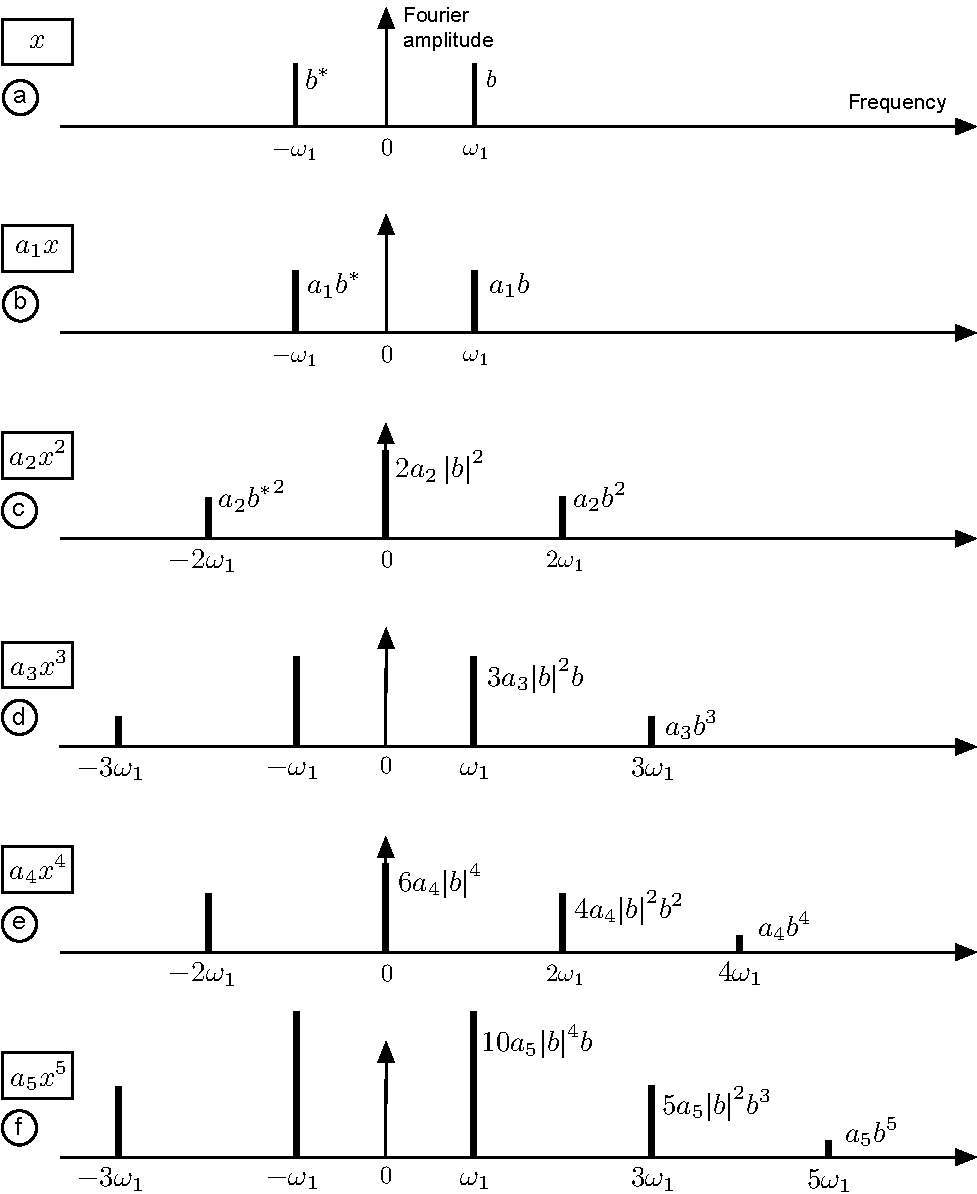
\includegraphics[width=0.9\linewidth]{fig/pa_1tone}
\caption [pa_1tone] 
{
\BL{Spectral effect of PA nonlinearity with single-tone test signal.}
Panel~(a) shows the spectrum of the sinusoidal input. The subsequent panels show schematically, and with variable vertical scale, the spectra of the first few terms in an polynomial PA model. Note especially how all ``odd-order'' (odd-$n$) terms $a_n x^n$ contribute to the spectrum at the fundamental frequency $\omega_1$. The linear contribution $a_1b$ is what one would like to have; the other contributions distort the amplified signal.
}
\label{Fig:pa_1tone}
\end{figure}


%--------------------
%:Fig:gaincompr_atan_gain
%--------------------
\begin{figure}
\centering
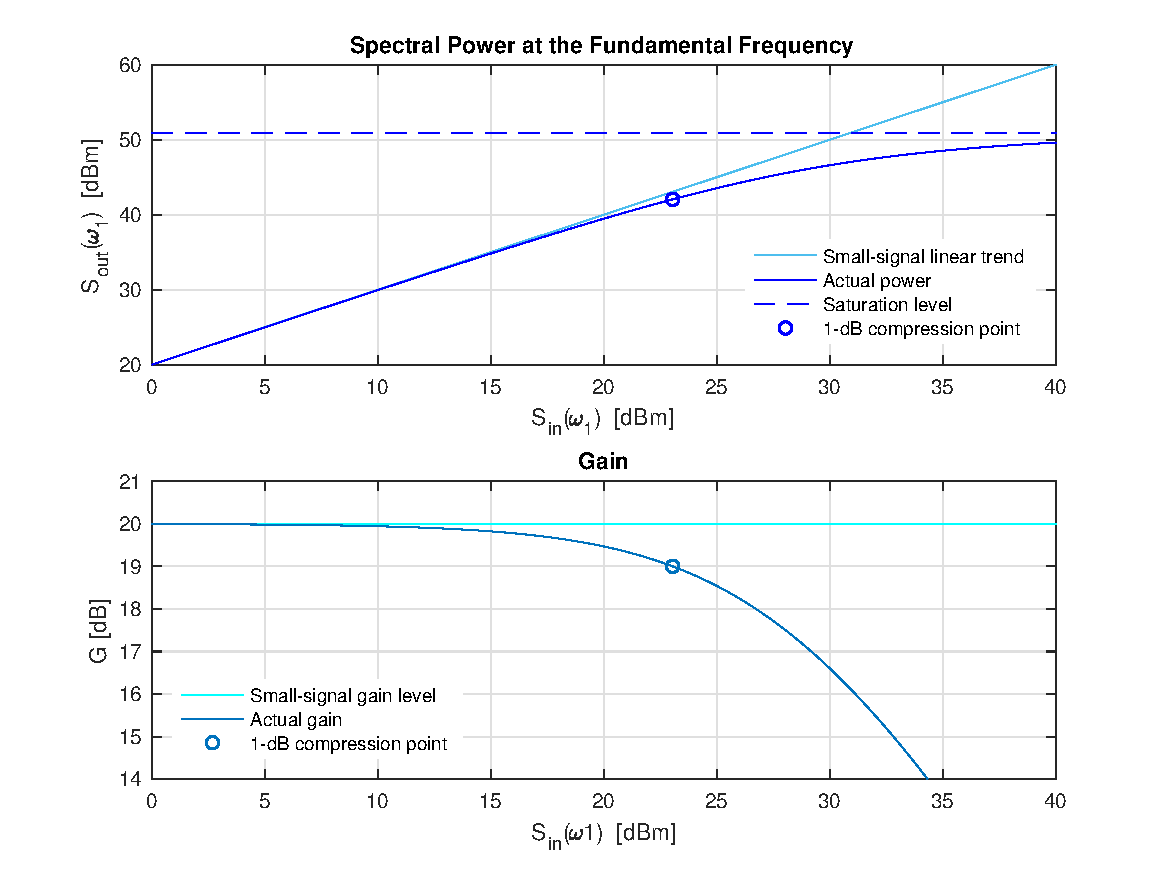
\includegraphics[width=1.0\linewidth]{fig/gaincompr_atan}
\caption [Gain compression with single-tone input.] 
{
\BL{Gain compression in our $\arctan$ toy model.} The top panel shows the output spectral power at the single-tone input frequency $\omega_1$, as function of the spectral power of the input signal. The output power saturates asymptotically to $S_\mr{ out}=50.9$~dBm. The bottom panel shows the amplifier gain $G = S_\mr{out}- S_\mr{in}$. The single-tone 1-dB compression point is marked both on the gain curve and the output power curve, at $S_\mr{in} = 23.0$~dBm. In the top panel, the small-signal linear trend is $G_0 + S_\mr{in}$. The small-signal power gain $G_0$ in the model is $20$~dB, and the ``voltage scale'' parameter $b_0$ is $27$~dBm ($5$~V). 
}
\label{Fig:gaincompr_atan}
\end{figure}


%--------------------
%:Fig:model_atan
%--------------------
\begin{figure}
\centering
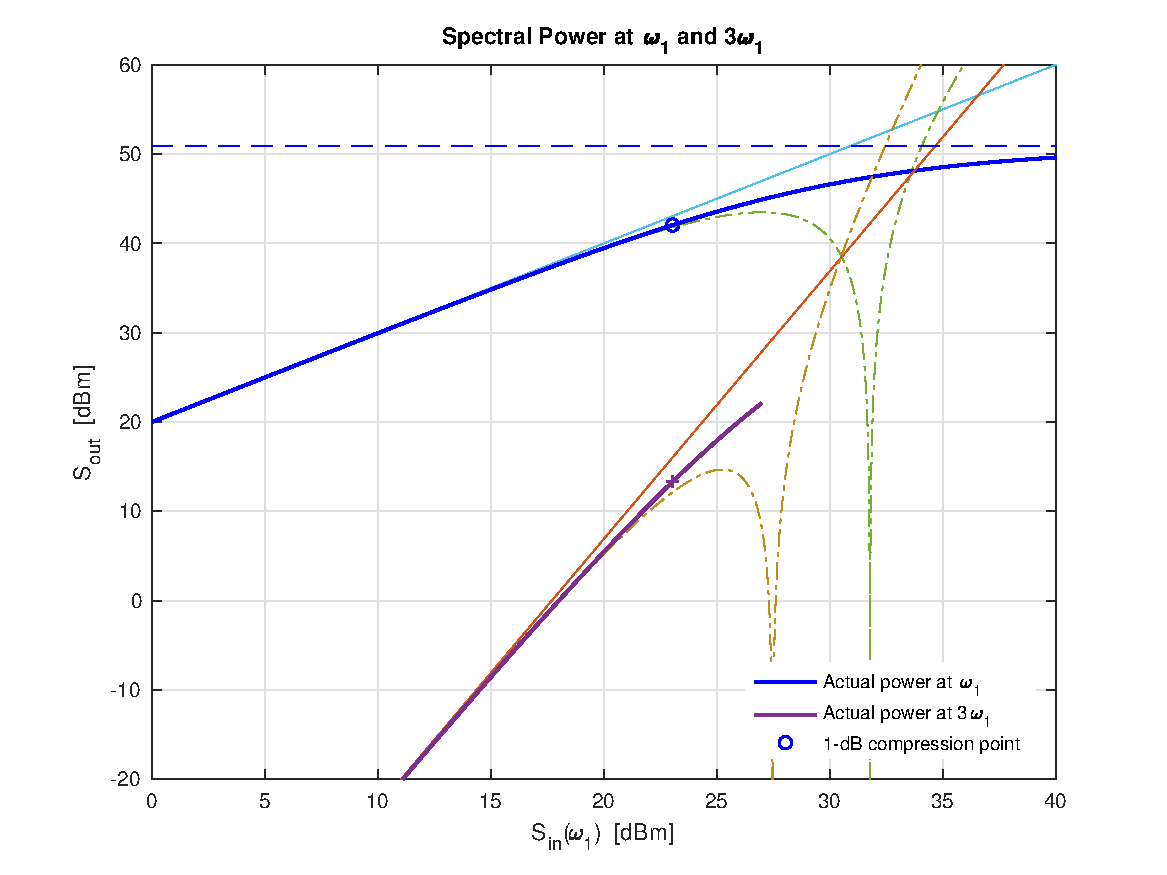
\includegraphics[width=1.0\linewidth]{fig/model_atan}
\caption [Single-tone spectrum in the $\arctan$ toy model.] 
{
\BL{Single-tone spectrum in the $\arctan$ toy model.}  
}
\label{Fig:model_atan}
\end{figure}



%--------------------
%:Fig:AFigure
%--------------------
\begin{figure}
\centering
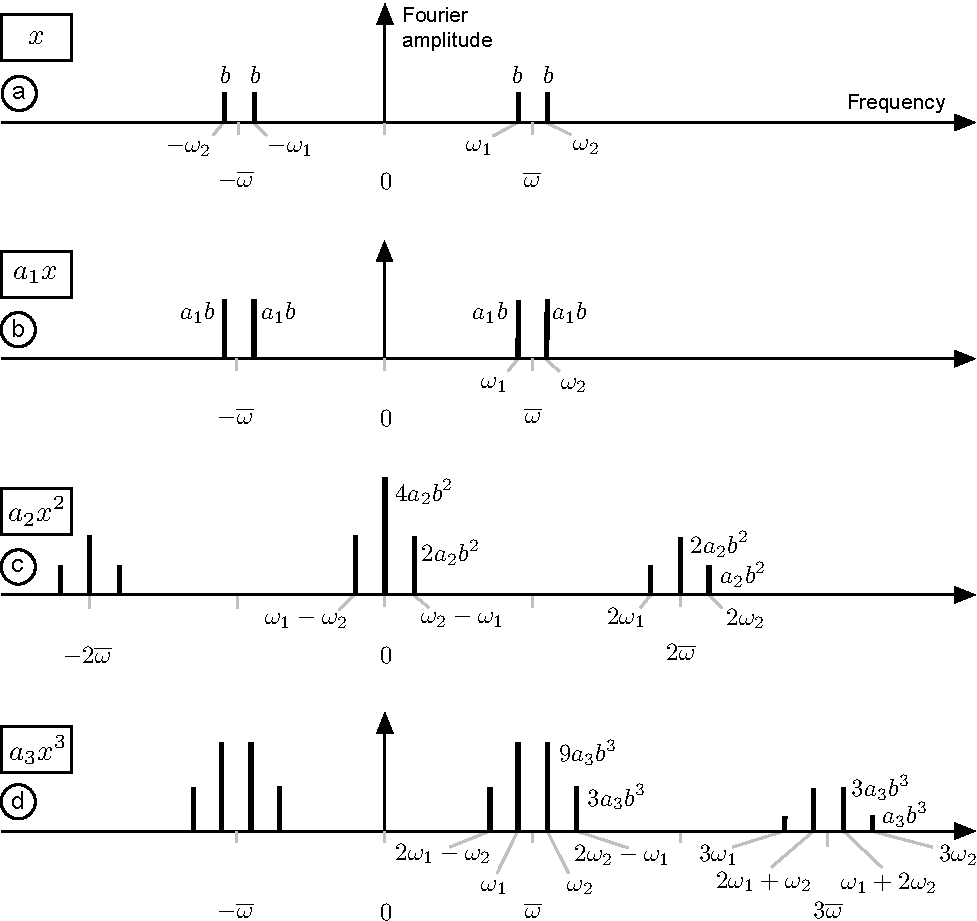
\includegraphics[width=0.9\linewidth]{fig/pa_3ic}
\caption [CAPTION TO LISTING] 
{
\BL{PA nonlinearities with two-tone test signal.}
}
\label{Fig:pa_3ic}
\end{figure}


%##############################################################################
\end{document}
%##############################################################################



